\section{Población y muestra}
\subsection{Población}
La población del presente estudio está conformada por \textbf{áreas de cultivo de caña de azúcar 
en la costa norte y centro del Perú}, desde el valle del Chira (Piura) hasta el valle Huaura (Lima).
Se obtuvo a partir del área de superficie agrícola en los valles de la costa proporcionada por MIDAGRI y la ubicación referencial de 
los ingenios azucareros (Ver figura \ref{fig:poblacion}).
 
\begin{figure}[H]
    \centering
    \caption{Áreas de cultivo de caña de azúcar.}
    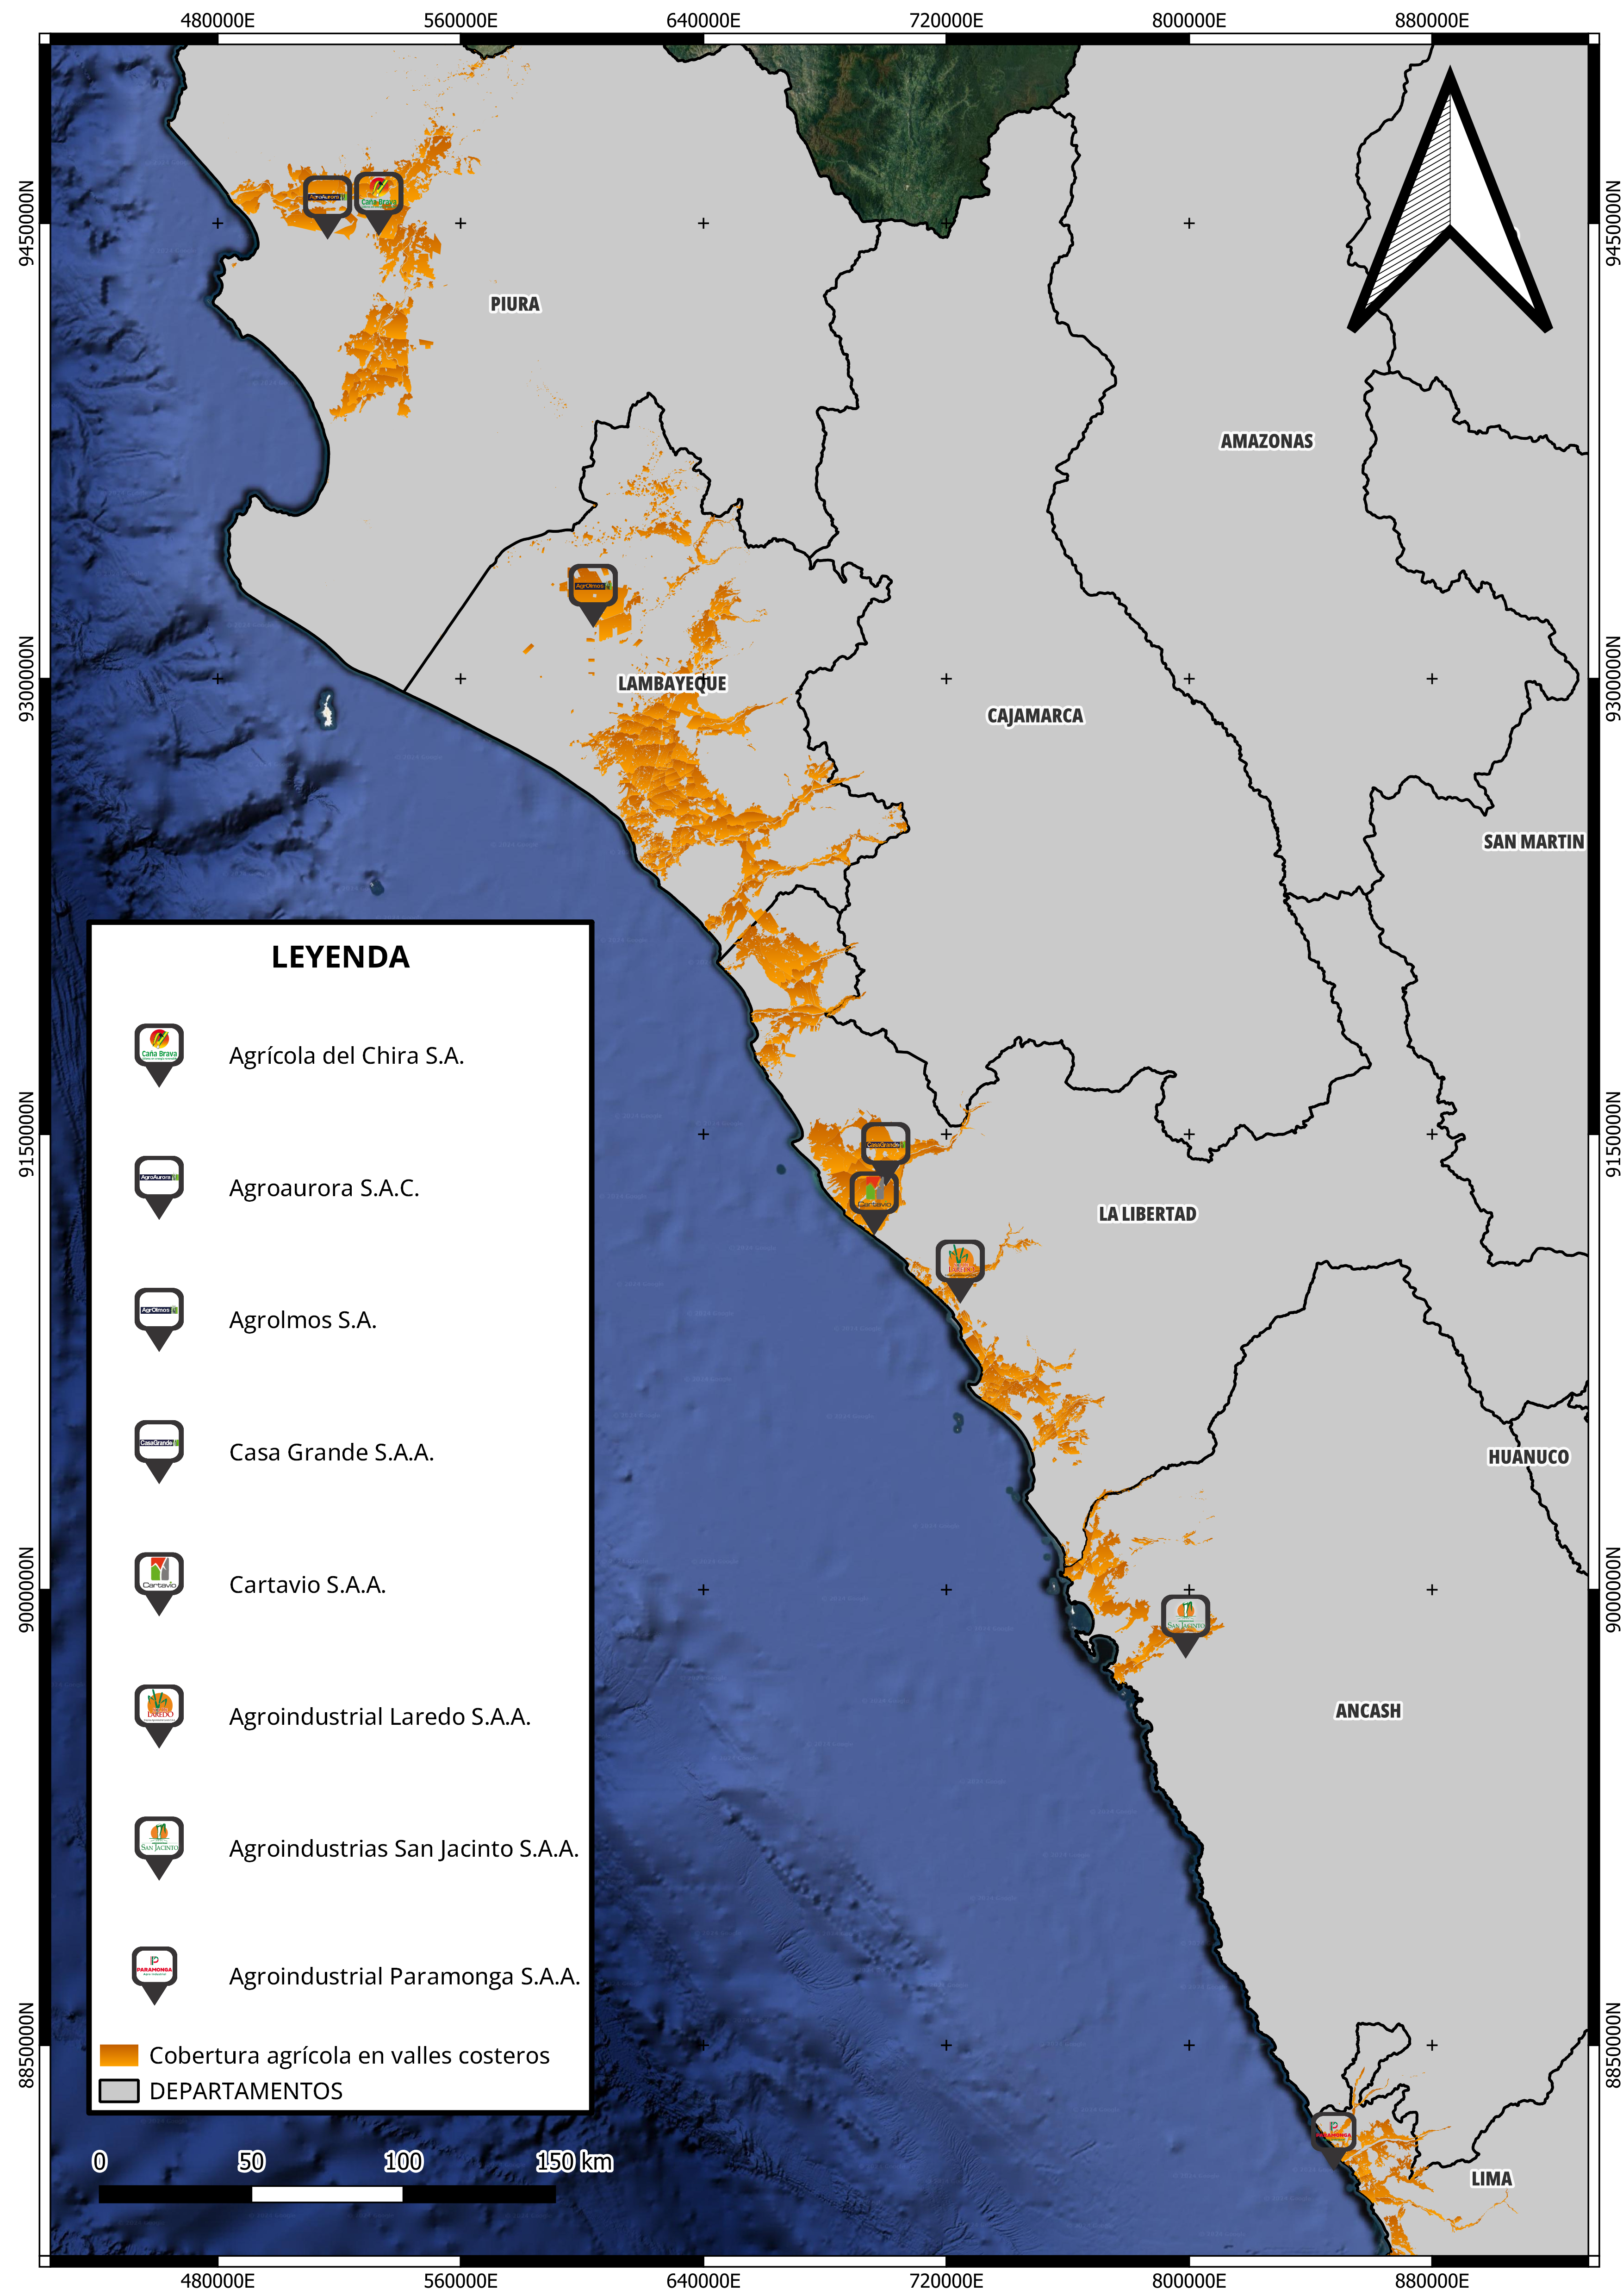
\includegraphics[width=0.6\textwidth]{img/6_metodologia/poblacion.png}
    \label{fig:poblacion}
    \begin{flushleft}
        \vspace{-\baselineskip}
        \textit{Nota.} Elaboración propia.        
        \vspace{-\baselineskip}
    \end{flushleft}
\end{figure}

En la Tabla \ref{tab:ingenios} se presentan los principales ingenios azucareros en la costa norte y centro del Perú, con su respectiva código administrado de la OEFA, ubicación y cuencas 
hidrográficas donde se encuentran.

\begin{table}[H]
    \centering
    \caption{Principales ingenios azucareros en la costa norte y centro del Perú.}
    \label{tab:ingenios}
    \begin{tabular}{p{3cm}p{2cm}p{2cm}p{4cm}p{3cm}}
        \hline
        \textbf{Empresa azucarera} & \textbf{Código administrado OEFA} & \textbf{Departamento} & \textbf{Cuencas Hidrográficas} & \textbf{Coordenadas del ingenio (lat, lon)} \\
        \hline
        \textbf{Agroaurora S.A.C.} & ADM17481 & Piura &  Cuenca Chira, Cuenca Piura e Intercuenca 1379. & (-4.929,-80.854) \\
        \textbf{Agrícola del Chira S.A.} & ADM16435 & Piura &  Cuenca Chira, Cuenca Piura e Intercuenca 1379. & (-4.918,-80.702) \\
        \textbf{Agrolmos S.A.} & ADM17036 & Lambayeque & Cuenca Olmos e Intercuenca 137779. & (-6.085,-80.063) \\       
        \textbf{Casa Grande S.A.A.} & ADM11828 & La Libertad & Cuenca Chicama, Intercuenca 137719 e Intercuenca 13773. & (-7.745,-79.186) \\
        \textbf{Cartavio S.A.A.} & ADM11829 & La Libertad & Cuenca Chicama. & (-7.892,-79.220) \\
        \textbf{Agroindustrial Laredo S.A.A.} & ADM11837 & La Libertad & Cuenca Chicama, Cuenca Moche e Intercuenca 137715. & (-8.094,-78.962) \\ 
        \textbf{Agroindustrias San Jacinto S.A.A.} & ADM11681 & Áncash & Cuenca Nepeña. & (-9.146,-78.281) \\
        \textbf{Agroindustrial Paramonga S.A.A.} & ADM11867 & Lima & Intercuenca 137591. & (-10.674,-77.823) \\
    \hline
    \end{tabular}
    \begin{flushleft}
        \textit{Nota.} Extraído del \href{https://sistemas.oefa.gob.pe/Portalpifa/IntervencionesUF.do}{Portal Interactivo de Fiscalización Ambiental} de OEFA.
        \vspace{-\baselineskip}
    \end{flushleft}    
\end{table}

\subsection{Muestra}
La muestra de este estudio está constituida por las \textbf{áreas donde se ha reportado la quema de caña de azúcar}, ubicadas en la costa norte y centro del Perú, desde los valles del Chira (Piura) hasta el valle del Huaura (Lima). Esta delimitación se basa en los reportes 
de quema provenientes del registro histórico de 471 emergencias ambientales relacionadas con esta práctica, en el período comprendido entre enero de 2020 y agosto 
de 2023, proporcionado por el OEFA (Figura \ref{fig:muestra}, parte 
izquierda).

\begin{figure}[H]
    \centering
    \caption{Áreas con reporte de quema de caña de azúcar (ROI's).}
    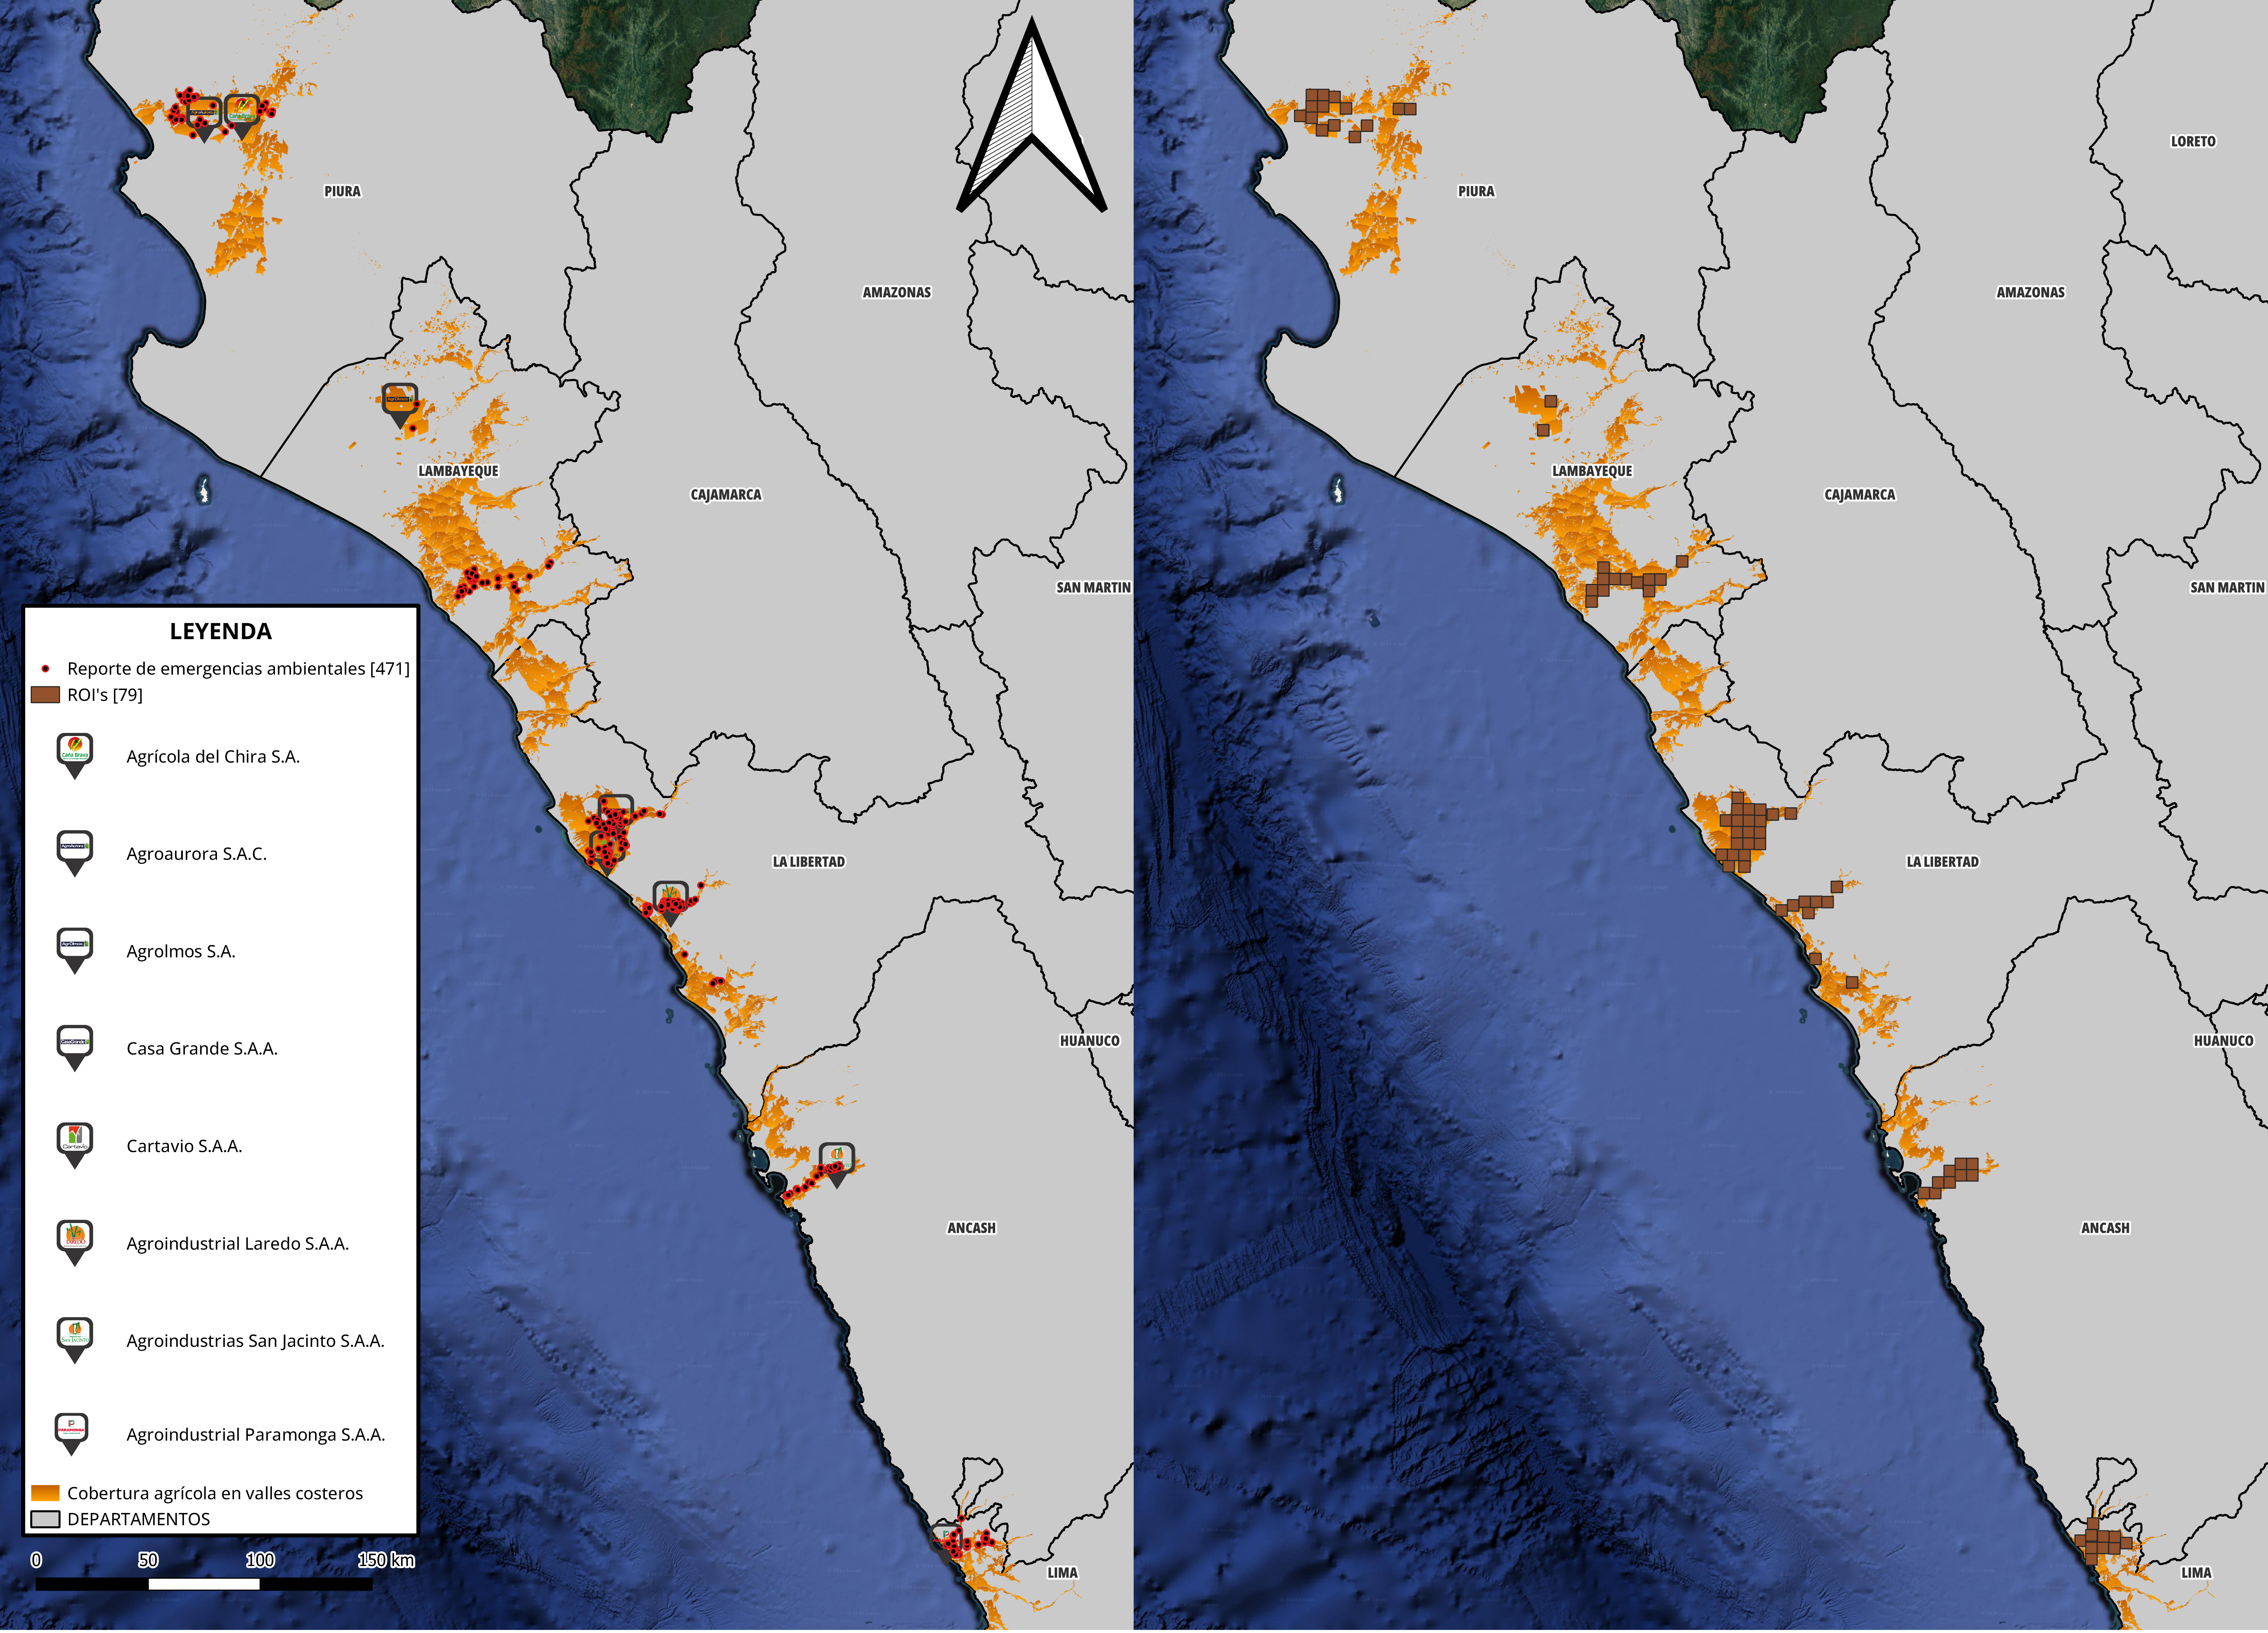
\includegraphics[width=1\textwidth]{img/6_metodologia/muestra.png}
    \label{fig:muestra}
    \begin{flushleft}
        \vspace{-\baselineskip}
        \textit{Nota.} Elaborado a partir del registro histórico de emergencias ambientales del OEFA.        
        \vspace{-\baselineskip}
    \end{flushleft}
\end{figure}


Como resultado, se generan incialmente 79 regiones de interés (ROI's), cada una correspondiente a una escena de imágenes Sentinel-2 L2A de $512 
\times 512$ con una resolución de píxel de 10 m por píxel (Figura \ref{fig:muestra}, parte derecha). 

En la Figura \ref{fig:figura_1} del Anexo, se muestra la tabla de los ROI's junto con sus coordenadas centrales y la cantidad de emergencias ambientales reportadas en cada uno de ellos.

    